\documentclass[tikz,border=10pt]{standalone}
\usepackage[utf8]{inputenc}
\usepackage{tikz, pgfplots}
\usetikzlibrary{positioning}
\usetikzlibrary{calc}

%https://latexdraw.com/tikz-shapes-circle/

\begin{document}

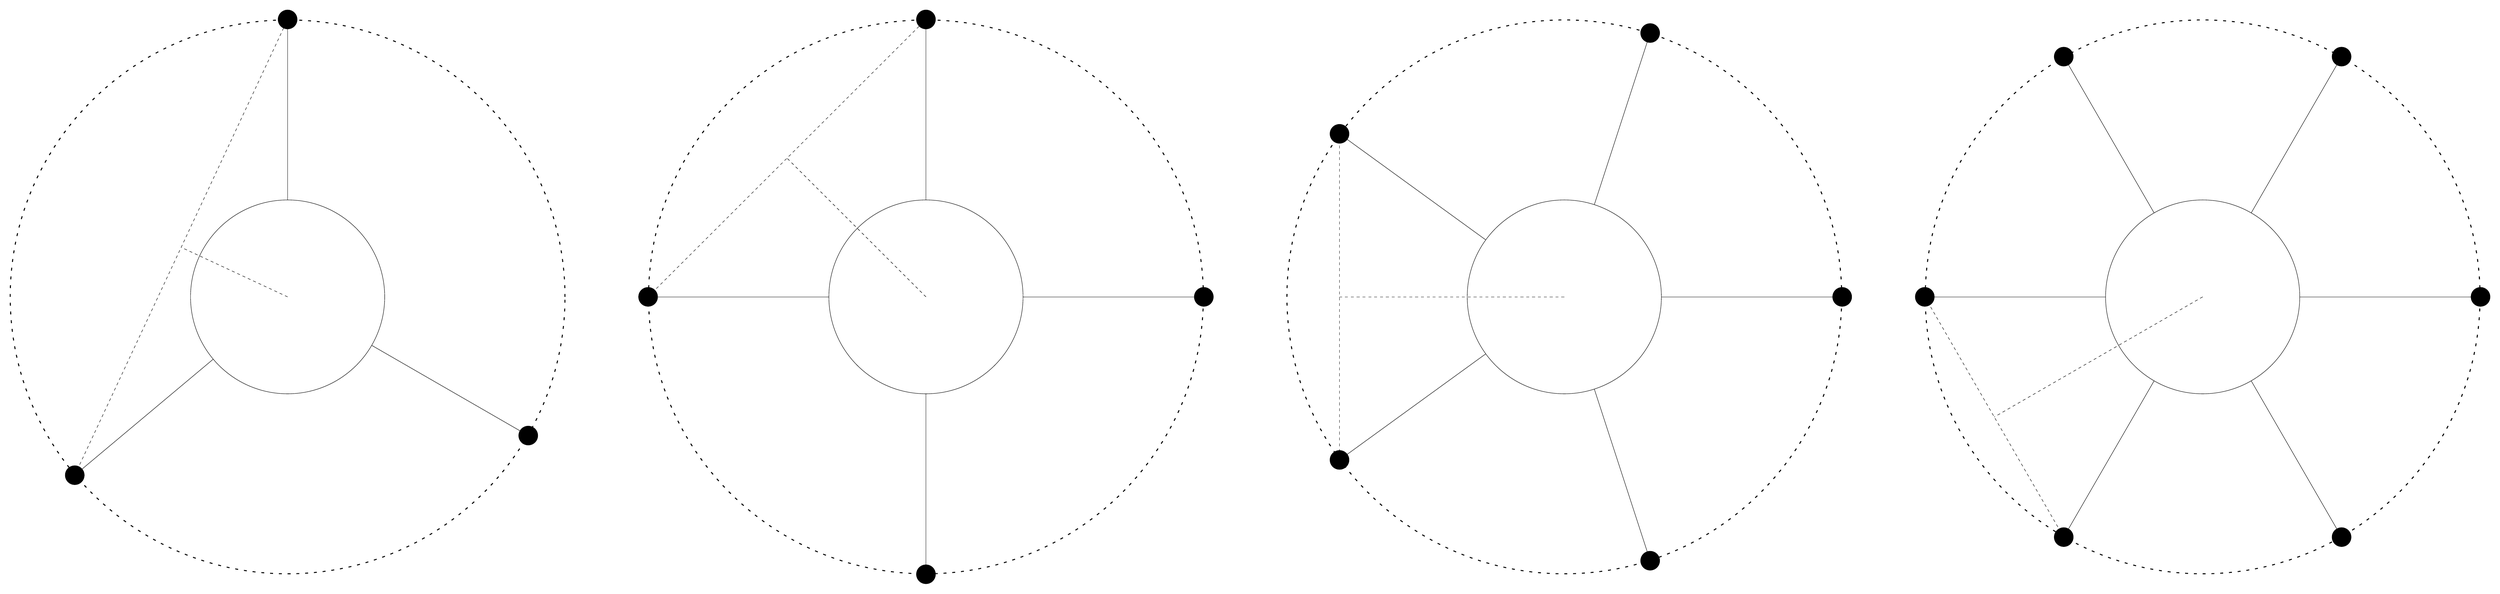
\begin{tikzpicture}[
base/.style ={circle,draw,minimum size = 7cm},
landing_radius/.style = {circle,draw,minimum size = 20cm,line width=1pt,dash pattern=on 3pt off 6pt}
]
\def\feet{10pt}

%Nodes
\node [base](3legs){};
\node [base](4legs) [right=of 3legs,xshift = 15cm] {};
\node [base](5legs) [right=of 4legs,xshift = 15cm] {};
\node [base](6legs) [right=of 5legs,xshift = 15cm] {};

\node [landing_radius](3legs_lr) at (3legs){};
\node [landing_radius](4legs_lr) at (4legs){};
\node [landing_radius](5legs_lr) at (5legs){};
\node [landing_radius](6legs_lr) at (6legs){};

%3 Legs
\draw (3legs.90) -- (3legs_lr.90);
\draw (3legs.-30)--(3legs_lr.-30);
\draw (3legs.220)--(3legs_lr.220);
\fill (3legs_lr.220) circle(\feet);
\fill (3legs_lr.-30) circle(\feet);
\fill (3legs_lr.90) circle(\feet);

%Effectice Landing 

\draw [dashed] (3legs_lr.220) -- (3legs_lr.90) node[scale = 2,midway,xshift = -0.75cm] {};


\coordinate (3legs_elr) at ($(3legs_lr.220)!0.5!(3legs_lr.90)$);

\draw [dashed] (3legs.center) -- (3legs_elr) {};


%4 Legs
\draw (4legs.90) -- (4legs_lr.90);
\draw (4legs.270)--(4legs_lr.270);
\draw (4legs.180)--(4legs_lr.180);
\draw (4legs.0)--(4legs_lr.0);

\fill (4legs_lr.90) circle(\feet);
\fill (4legs_lr.270) circle(\feet);
\fill (4legs_lr.180) circle(\feet);
\fill (4legs_lr.0) circle(\feet);

%Effectice Landing 

\draw [dashed] (4legs_lr.180) -- (4legs_lr.90){};

\coordinate (4legs_elr) at ($(4legs_lr.180)!0.5!(4legs_lr.90)$);

\draw [dashed] (4legs.center) -- (4legs_elr) {};


%5 Legs
\draw (5legs.72) -- (5legs_lr.72);
\draw (5legs.144)--(5legs_lr.144);
\draw (5legs.216)--(5legs_lr.216);
\draw (5legs.288)--(5legs_lr.288);
\draw (5legs.360)--(5legs_lr.360);

\fill (5legs_lr.72) circle(\feet);
\fill (5legs_lr.144) circle(\feet);
\fill (5legs_lr.216) circle(\feet);
\fill (5legs_lr.288) circle(\feet);
\fill (5legs_lr.360) circle(\feet);

%Effectice Landing 

\draw [dashed] (5legs_lr.144) -- (5legs_lr.216){};

\coordinate (5legs_elr) at ($(5legs_lr.144)!0.5!(5legs_lr.216)$);

\draw [dashed] (5legs.center) -- (5legs_elr) {};


%6 Legs
\draw (6legs.60) -- (6legs_lr.60);
\draw (6legs.120)--(6legs_lr.120);
\draw (6legs.180)--(6legs_lr.180);
\draw (6legs.240)--(6legs_lr.240);
\draw (6legs.300)--(6legs_lr.300);
\draw (6legs.360)--(6legs_lr.360);

\fill (6legs_lr.60) circle(\feet);
\fill (6legs_lr.120) circle(\feet);
\fill (6legs_lr.180) circle(\feet);
\fill (6legs_lr.240) circle(\feet);
\fill (6legs_lr.300) circle(\feet);
\fill (6legs_lr.360) circle(\feet);

%Effectice Landing 

\draw [dashed] (6legs_lr.180) -- (6legs_lr.240){};

\coordinate (6legs_elr) at ($(6legs_lr.180)!0.5!(6legs_lr.240)$);

\draw [dashed] (6legs.center) -- (6legs_elr) {};






\end{tikzpicture}

\end{document}